\documentclass{article}
\usepackage{graphicx}
\usepackage{fullpage} % really need smaller margins for two column steps
\usepackage[none]{hyphenat} %no hyphenation!
\usepackage{verbatim} %for the comment environment

%\usepackage{array}
%\setlength\extrarowheight{3pt}

% I have no idea how this works! But it allows for two column lists... somehow
% http://tex.stackexchange.com/questions/89603/horizontal-enumeration-in-multiple-columns
\usepackage{paralist}
\usepackage{tabto}
\usepackage{etoolbox}
%\newenvironment{twocol}
% {\NumTabs{2}\inparaenum\let\latexitem\item
%  \def\item{\def\item{\tab\latexitem}\latexitem}}
% {\endinparaenum}

% al is like description but nice and aligned
% http://tex.stackexchange.com/questions/67720/description-list-with-aligned-descriptions
\usepackage{calc}  
\usepackage[shortlabels]{enumitem} %without 'shortlabels' enumerate is sad
\newenvironment{al}
{\begin{description}[leftmargin=!,labelwidth=\widthof{\bfseries Preconditions:}]}
{\end{description}}

% Gosh fracking darn it it was hard to get a working two column layout that
%  allowed multiple lines.
% LaTeX complains, but whatever I'm a newbie and have no idea what I'm doing
% and actually did something besides copy snippets off stackoverflow! Amazing!
\newcounter{twocoli}
\newenvironment{twocol}
{ \setcounter{twocoli}{1}
  \begin{tabular}{ p{0.45\textwidth} p{0.43\textwidth}} }
{ \end{tabular} }
\newcommand{\tabrow}[2]
{   \arabic{twocoli}. \  \parbox[t]{0.40\textwidth}{#1 \vspace{0.1 in}} \stepcounter{twocoli} 
  & \arabic{twocoli}. \  \parbox[t]{0.47\textwidth}{#2 \vspace{0.1 in}} \stepcounter{twocoli}\\}
\newcommand{\tableft}[1]
{   \arabic{twocoli}. \  \parbox[t]{0.40\textwidth}{#1 \vspace{0.1 in}} & \parbox[t]{0.47\textwidth}{ \vspace{0.1 in}} \stepcounter{twocoli}\\}
\newcommand{\tabright}[1]
{ - & \arabic{twocoli}. \  \parbox[t]{0.40\textwidth}{#1 \vspace{0.1 in}} \stepcounter{twocoli}\\}
% ------------------------------------------------------------------------------
\begin{document}



\section*{Use Case Diagram}
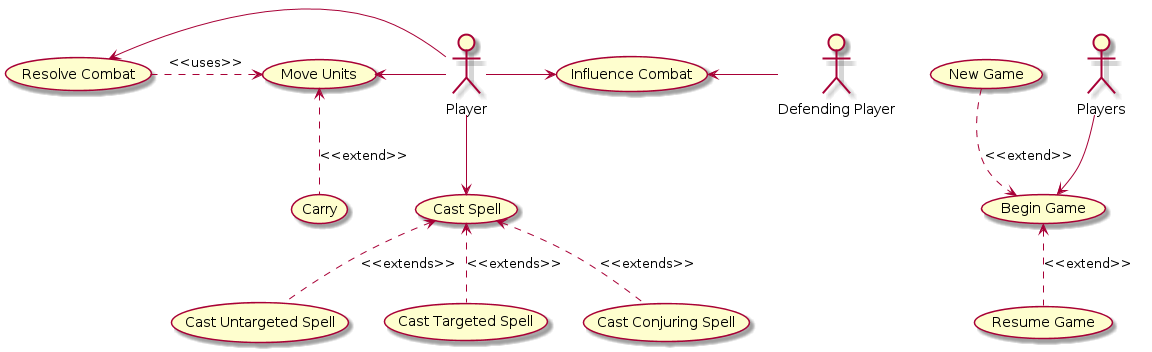
\includegraphics{use_cases.png}

\tableofcontents

%Generic Use-Case
\begin{comment}

\section{}
\begin{al}
	\item[Actor:] Player
	\item[Goal:]
	\item[Precondition:]
	\item[Summary:]
\end{al}
\textbf{Steps:} \\
\begin{twocol}
  \tableft{}
  \tabrow{}
         {}
\end{twocol}
\begin{al}
	\item[Alternatives:]
	\begin{enumerate}
	\item
	\item
	\item
	\end{enumerate}
\end{al}

\end{comment}

\begin{comment}

* Select Game Type, Select Scenario overlap and should be merged
  Resume game could extend or be merged with a start game use case

* We have save game but not quit. Is save game related enough to quitting
  to extend or be merged with quitting?

* Should Choose Leader be merged with a general "Select Unit(s)"?

* Should enemy player be an actor in combat?

* Display Random Event & Player order could use more User Actions
  to make it use-casey. "Actor: System" is the sort of thing that would give
  Dr. Jeffery a heart-attack

* Invasion can happen outside of normal player movement
  And the player might not be able to prevent it.

* Is confirm important enough to be it's own use case? Or should it just be
  part of the steps of other use cases?

* Some things don't fit nicely into the two-column format. do they need tweaking?

* View Character Statistics should maybe be expanded to any unit type, and include
  any current effects such as current Movement Points.

* Should Advance and Retreat extend Movement? Extend Combat?

  Overall I feel like we could have more extending, to make an interesting diagram

* are we missing any big use-cases? Do any need to be tweaked

Need plan of action to have diagram and associated descriptions ready on thursday

\end{comment}

\section{Select Game Type}
\begin{al}
	\item[Actor:] Player starting the game
	\item[Goal:] To resume a game or start a new game
	\item[Summary:] Player selects options from a menu, choosing what game to initate.
\end{al}
\textbf{Steps:} \\
\begin{twocol}
  \tabrow{Player selects "new game".}{System displays a list of scenarios.}
  \tableft{Player selects a scenario.}
\end{twocol}
\begin{al}
	\item[Alternative:] Player selects load game. In this case player selects
                        from a list of saved games.
\end{al}

\section{Set up a scenario}
\begin{al}
	\item[Actor:] Players starrting a game
	\item[Goal:] To do scenario set-up
	\item[Summary:] Player selects a faction and places the allocated units in valid hexes.
\end{al}
\textbf{Steps:} \\
\begin{twocol}
  \tabright{System displays a list of factions.}
  \tabrow{Player chooses from the list of factions.}
         {System displays faction information such as victory conditions and
          starting units, prompts player to confirm selection.}
  \tabrow{Player confirms selection.}
         {System displays units to be placed and valid hexes.}
  \tabrow{Player selects units and places them in appropriate hexes until all
          available units have been placed.}
         {System prompts for confirmed placement.}
  \tableft{Player confirms and scenario begins.}
\end{twocol}
\begin{al}
	\item[Alternatives:]
	\begin{enumerate}
	\item Player cancels faction selection, system allows player to pick another faction.
	\item Player cancels unit placement. System resets last unit placement.
	\end{enumerate}
\end{al}

\section{Resume Game} %should this be part of "Start Game"?
\begin{al}
	\item[Actor:] Player
	\item[Goal:] To resume a saved game
	\item[Precondition:] A saved game exists. The player is at the proper menu
	                     to select it. %Second sentence seems to focus on interface a lot
	\item[Summary:] The player restores a previously saved state
	\item[Related:] \textbf{Confirm}
\end{al}
\textbf{Steps:} \\
\begin{twocol}
  \tabrow{The player selects the "Resume Game" option.}
	     {The system displays the available saved games.}
  \tabrow{The player selects the desired save file.}
         {The system displays a prompt.} 
  \tabright{The system loads the saved state.}
\end{twocol}

\section{Save Game} %Should "Quit Game" extend this?
\begin{al}
	\item[Actor:] Player
	\item[Goal:] To save the current game state for later play
	\item[Precondition:] A game is currently being played
	\item[Summary:] The player selects a save option and the system saves
	                the current state.
	\item[Related:] \textbf{Confirm}
\end{al}
\textbf{Steps:} \\
\begin{twocol}
  \tabrow{The player selects the "Save Game" option.}
         {The system displays a list of available save slots.} %Not file folder?
  \tabrow{The player selects the desired slot.}
         {The system displays the relevant confirmation prompt.}
  \tabright{The system saves the current state of the game.}
\end{twocol}

\section{Select Scenario} %Should this be part of "Begin Game"?
\begin{al}
	\item[Actor:] Hosting Player
	\item[Goal:] To select a pre-made game scenario.
	\item[Precondition:] A new game has been initiated
	\item[Summary:] The hosting player selects a pre-made game scenario, for a new game.
	\item[Related:] \textbf{Confirm}
\end{al}
\textbf{Steps:} \\
\begin{twocol}
  \tabright{The system displays the list of available pre-made scenarios for the
            hosting player to select.}
  \tabrow{The player selects the desired scenario from the list.}
         {The system displays the relevant confirmation prompt.}
  \tabright{The system loads the selected scenario.}
\end{twocol}


\section{End Inter-Phase}
\begin{al}
	\item[Actor:] Player
	\item[Goal:] To end the current player's phase.
	\item[Precondition:] The game is in a phase the player has control to end.
	\item[Summary:] The player wishes to end their current phase early. If the
                    rules are not violated the turn is ended.
	\item[Related:] \textbf{Confirm}
\end{al}
\textbf{Steps:} \\
\begin{twocol}
  \tabrow{The player selects an "End Phase" option}
         {The system displays the relevant confirmation prompt.}
  \tabright{The system ends the current phase.}
\end{twocol}

\section{Select Ally Candidate}
\begin{al}
	\item[Actors:] All Players
	\item[Goal:] To determine player alliances for the game-turn.
	\item[Precondition:] It is currently the player-Order Determination Inter-Phase.
	\item[Summary:] Each player selects any other player(s) they would like to
                    be allied with for the turn. 
\end{al}
\textbf{Steps:} \\
\begin{twocol}
  \tabright{The system displays to each player a list of potential allies
            (the other, eligible, players).}
  \tableft{The players select any other player(s) they wish to ally with for the game-turn.}
  \tabrow{The player indicates they are finished selecting hopeful allies.}
         {The system moves to the next phase.}
\end{twocol}

\section{Display Random Event and Player Order}
\begin{al}
    % Players should probably be an actor
    % If it's just a display without any interaction it could be a step of a larger use case
	\item[Actor:] System 
	\item[Goal:] Display the game-turn's random event to all players
	\item[Precondition:] The previous game-turn has ended and the system has
                         determined the random event and player order for the
                         next game turn.
	\item[Summary:] The system displays the random event and player order to all
                    players for a period of time.
\end{al}
\textbf{Steps:} \\
\begin{twocol}
	\begin{enumerate}
  \item The system displays the random event and a description of the event and its effects 
        for an interval of time
  \item The system replaces the random even display with the player order display for an 
        interval of time. This includes alliances.
	\end{enumerate}
\end{twocol}

\section{Move Units}
\begin{al}
	\item[Actor:] Player
	\item[Goal:] To move unit(s) from one tile to another
	\item[Summary:] Move a unit, character, monster, stack, or subset of a stack
                    from a starting tile to a destination tile, depending on
                    terrain or movement points.
    \item[Precondition:] It is the player's movement phase
	\item[Related:] \textbf{Carry} \textbf{Select Subset of Stack}
\end{al}
\textbf{Steps:} \\
\begin{twocol}
  \tabrow{The player selects a unit, character, monster, stack, or stack subset.}
         {The system displays what hexes are reachable by those unit(s) based
          on their remaining Movement Points.}
  \tabrow{The player selects a destination hex to move the unit(s) to.}
         {The unit(s) are moved and their movement points are subtracted accordingly.}
\end{twocol}
\begin{al}
	\item[Alternatives:]
	\begin{enumerate}
	    \item If unit is moved into an enemy zone of control, it's movement might
              immediately end.
		\item The user can cancel movement after being shown the reachable hexes.
		\item Some unit(s) will not be able to make a valid movement for various
		      reasons, in this case the user must cancel the movement.
	\end{enumerate}
\end{al}

\section{Carry}
\begin{al}
	\item[Actor:] Player
	\item[Goal:] To carry a character using a flying unit
	\item[Summary:] Flying units or monsters can carry other characters if said
                    other characters haven't moved yet.
    \item[Precondition:] It is the movement phase and the player has a flying
                         unit that has room on it's back, 
                         in range of a character that hasn't moved yet
	\item[Related:] \textbf{Movement}
\end{al}
\textbf{Steps:} \\
\begin{twocol}
	\tabrow{The player moves a flying unit over unmoved character(s) as per
            \textbf{Movement}}
           {The system asks which, if any, characters should be carried.}
	\tabrow{The player indicates which, if any, characters they want carried.}
           {Those characters are stacked with the flying unit for the remainder
            of the movement phase.}
\end{twocol}
    
\section{Select Subset of Stack}
\begin{al}
	\item[Actor:] Player
	\item[Goal:] To select one or more units out of a stack
	\item[Summary:] There's lots of unit stacking in Swords \& Sorcery. 
                    The player needs an easy way to both use a stack as a whole
                    or to use specific units from a stack.
\end{al}
\textbf{Steps:} \\
\begin{twocol}
  \tabrow{The user selects a stack.}
         {The user is given the choices of using the stack as a whole,
          selecting one or more units out of the stack,
          or cancelling the selection.
          }
  \tabrow{The user either cancels or selects the desired unit(s).}
         {Those units become selected.}
  \tableft{The user continues on with whatever action they were going to do
           using the selected units.}
\end{twocol}
\begin{al}
	\item[Alternatives:]
	\begin{enumerate}
	\item In some states it might only make sense to select a single unit
          out of a stack. In this case the user is not given the choice of
          selecting multiple units or the whole stack
	\item In some states such as \textbf{Eliminate Unit} the player may be forced
          to select some number of units. In this case there is no option to cancel
	\end{enumerate}
\end{al}


\section{Attack Units} %section 13
\begin{al}
	\item[Actor:] Player %, Enemy Player
	\item[Goal:] Attack opposing player through combat
	\item[Precondition:] Player is in the Combat Resolution Segment
	\item[Summary:] Player selects units to attack and unit to be attacked.
	                Combat is resolved by the system.
	\item[Related:] \textbf{Choose Leader}, \textbf{Spend Combat Mana}
\end{al}
\textbf{Steps:} \\
\begin{twocol}
  \tableft{Attacker selects units to attack.}
  \tabrow{Attacker selects unit to be attacked.}
         {System notifies defending player.}
  \tableft{If multiple leaders (Choose Leader).}
  \tabrow{If magic capable leaders (Spend Combat Mana).}
         {System displays effects of combat.}
\end{twocol}
\begin{al}
	\item[Alternatives:] 
	\begin{enumerate} \item User deselects units in step 1.
                      \item Combat is not valid in step 2.
	\end{enumerate}
\end{al}

\section{Advance Units After Combat}
\begin{al}
	\item[Actor:] Player
	\item[Goal:] To move units forward into the enemies retreating path
	\item[Precondition:] Player has won combat
                         and opposing player has retreated units.
	\item[Summary:] Player can choose to move units into retreating path
                    of enemy after combat.
\end{al}
\textbf{Steps:} \\
\begin{twocol}
  \tableft{Player selects units to advance.}
  \tabrow{Player selects path of advance.}
         {System checks if path is valid and displays result.}
\end{twocol}
\begin{al}
	\item[Alternatives:] 
	\begin{enumerate} \item Player chooses not to move.
                      \item Player deselects units in step 1.
                      \item Path is not valid so unit does not move.
	\end{enumerate}
\end{al}

\section{Retreat}
\begin{al}
	\item[Actor:] Player
	\item[Goal:] To retreat units after losing combat
	\item[Precondition:] Player has just lost combat
	\item[Summary:] The player can choose to retreat units after combat or kill off units.
\end{al}
\textbf{Steps:} \\
\begin{twocol}
  \tableft{System shows player units to be retreated.}
  \tableft{Player selects units to kill.}
  \tabrow{Player chooses path for remaining units.}
         {System checks if path is valid and displays results.}
\end{twocol}
\begin{al}
	\item[Alternatives:]
	\begin{enumerate} \item Units are all killed in combat.
                      \item Player kills all units in step 2.
                      \item Path not valid in step 3
	\end{enumerate}
\end{al}

\section{Choose Leader}
\begin{al}
	\item[Actor:] Player
	\item[Goal:] To select one leader if multiple are present
	\item[Precondition:] Player has more than one leader.
	\item[Summary:] Player chooses which leader to use.
\end{al}
\textbf{Steps:} \\
\begin{twocol}
  \tabrow{Player selects leader from stack.}
         {System shows player which leader is to be used.}
\end{twocol}
\begin{al}
	\item[Alternative:] Player deselects unit in step 1.
                        Leader is not allowed to be used.
\end{al}

\section{Spend Combat Mana}
\begin{al}
	\item[Actor:] Player
	\item[Goal:] Cast magic from leaders in combat
	\item[Precondition:] Player is in combat and has magical leader
                         with mana points
	\item[Summary:] Player chooses which leader to use.
\end{al}
\textbf{Steps:} \\
\begin{twocol}
  \tableft{Player selects character.}
  \tabrow{Player chooses amount of mana to spend.}
         {System shows player combat strength of spell.}
\end{twocol}
\begin{al}
	\item[Alternatives:]
	\begin{enumerate} \item Player deselects unit in step 1.
                      \item Player does not have enough mana in step 2.
	\end{enumerate}
\end{al}

\section{Rally Units}
\begin{al}
	\item[Actor:] Player
	\item[Goal:] Attempt to rally units that have been demoralized
	\item[Precondition:] Player has demoralized units and leader is present in stack. player in Unit Rallying Segment of Army Combat Phase
	\item[Summary:] Player chooses leader to use if multiple and is shown if
	                rally was passed. %wording seems kinda confusing, what is passed?
\end{al}
\textbf{Steps:} \\
\begin{twocol}
  \tableft{Player selects demoralized units to be rallied.}
  \tabrow{Player selects leader to rally with, if there are more than one.}
         {System shows result of rally.}
\end{twocol}
\begin{al}
	\item[Alternatives:]
	\begin{enumerate} \item Player deselects units in step 1.
                      \item Leader is not allowed to be used.
	                  \item Units cannot be rallied.
	\end{enumerate}
\end{al}

%magic
\section{View Character Statistics}
\begin{al}
	\item[Actors:] Player
	\item[Goal:] view the statistics and current state of a certain character 
            or monster in play. 
	\item[Precondition:] a character or monster is in play.
	\item[Summary:] The user performs this action when he wishes to view the full statistics
            relating to a character or monster in play. It is similar to consulting the character’s 
            card in the manual system.
\end{al}
\textbf{Steps:} \\
\begin{twocol}
  \tabrow{Player selects the character or monster}
         {System displays a menu asking what the user wants to do with the character or monster
(may include Move, Attack, Cast spell, View, etc\ldots depending on game phase).}
  \tabrow{ Player chooses View.}
         { System displays the character or monster’s relevant statistics (those on the game card
      plus manna level if applicable) in a new window}
  \tableft{User closes the window.}
\end{twocol}
\begin{al}
	\item[Alternative:] User can choose Cancel instead in Step 3 to close the menu.
\end{al}

\section{Cast Untargeted Spell}
\begin{al}
        \item[Actors:] Player
        \item[Goal:] To cast a particular spell on a particular target, which may be a
            group of hexes, hex sides, characters, or units.
        \item[Precondition:] Player fulfills a set of preconditions for at least one
            spell. These preconditions depend on the characters available, their manna
            levels, and the game phase.
        \item[Summary:] The actor will choose one of his characters, and select a spell.
\end{al}
\textbf{Steps:} \\
\begin{twocol}
  \tabrow{ Player selects one of his or her characters with a mouse click}
         {  System displays a menu asking what the user wants to do with the character (may
include Move, Attack, Cast spell, View, etc. . . depending on game phase).}
  \tabrow{ Player chooses Cast spell.}
         { System displays a window listing all spells that the character is capable of attempting
given its Magic Power Level, current Manna points, the game phase, which types of
spells the character has cast that turn, and how many game-turns are left in the game
play.}
  \tabrow{ User selects one of the untargetted spells.}
         { System calculates the result if the character was attempting a higher order spell, then
makes internal adjustments to create the force walls.}
  \tabright{System reports the spell’s results in a dialog box.}
  \tableft{ User accepts results, closing dialog box.}
\end{twocol}
\begin{al}
        \item[Alternative:] User may choose to cancel in steps 3, or 5.
\end{al}


\section{Cast Targeted Spell}
\begin{al}
        \item[Actors:] Player
        \item[Goal:] To cast a particular spell on a particular target, which may be a 
            group of hexes, hex sides, characters, or units.
        \item[Precondition:] Player fulfills a set of preconditions for at least one 
            spell. These preconditions depend on the characters available, their manna 
            levels, the targets available, and the game phase.
        \item[Summary:] The actor will choose one of his characters, select a spell, 
            and then choose one or more targets based on the cost of the spell.
\end{al}
\textbf{Steps:} \\
\begin{twocol}
  \tabrow{ Player selects one of his or her characters with a mouse click}
         {  System displays a menu asking what the user wants to do with the character (may
include Move, Attack, Cast spell, View, etc. . . depending on game phase).}
  \tabrow{ Player chooses Cast spell.}
         { System displays a window listing all spells that the character is capable of attempting
given its Magic Power Level, current Manna points, the game phase, which types of
spells the character has cast that turn, and how many game-turns are left in the game
play.}
  \tabrow{ User selects one of the targetted spells.}
         { System highlights possible target hex sides and asks the user to choose one.}
  \tabrow{ User selects up to as many of the specific type of target as his character 
     can afford to cast the spell on at a cost of 2 Manna points per hex side. When 
     done, user can press continue.}
         { System calculates the result if the character was attempting a higher order spell, then
makes internal adjustments to create the force walls.}
  \tabright{System reports the spell’s results in a dialog box.}
  \tableft{ User accepts results, closing dialog box.}
\end{twocol}
\begin{al}
        \item[Alternative:] User may choose to cancel in steps 3, 5, or 7.
\end{al}



\section{Cast Conjuring Spell}
\begin{al}
        \item[Actors:] Player
        \item[Goal:] To conjure a particular type of unit to aide the player.
        \item[Precondition:] It must be the player's Magic phase. The user must have a 
            character of attempting a conjuring spell and have Manna points for it. 
            No non-conjuring spells may have been cast by this character this game-turn.
        \item[Summary:] The actor will choose one of his characters, select a spell,
            and then choose how long the unit is to remain in play.
\end{al}
\textbf{Steps:} \\
\begin{twocol}
  \tabrow{ Player selects one of his or her characters with a mouse click}
  {  System displays a menu asking what the user wants to do with the character (may
include Move, Attack, Cast spell, View, etc. . . depending on game phase).}
  \tabrow{ Player chooses Cast spell.}
   { System displays a window listing all spells that the character is capable of attempting
given its Magic Power Level, current Manna points, the game phase, which types of
spells the character has cast that turn, and how many game-turns are left in the game
play.}
  \tabrow{ User selects one of the targetted spells.}
   { System highlights possible target hex sides and asks the user to choose one.}
  \tabrow{ User selects up to as many game-turns as he can afford, given the cost of the 
      spell.}
   { System calculates the result if the character was attempting a higher order spell, then
makes internal adjustments to create the force walls.}
  \tabright{System reports the spell’s results in a dialog box.}
  \tableft{ User accepts results, closing dialog box.}
\end{twocol}
\begin{al}
        \item[Alternative:] User may choose to cancel in steps 3, 5, or 7.
\end{al}

\section{Manna Transfer}
\begin{al}
        \item[Actors:] Player
        \item[Goal:] To transfer Manna between a player's characters.
        \item[Precondition:] It must be this player’s Magic phase, and the user must have a character
capable of attempting a first level spell, and this character must have 2 Manna points.
Another of the player’s magic-capable characters must reside in the same hex as the casting
character.
        \item[Summary:] the user selects a character, chooses this spell, and then selects how much
Manna to transfer and to what character.
\end{al}
\textbf{Steps:} \\
\begin{twocol}
                  \tabrow{ Player selects one of his or her characters}
                  { System displays a menu asking what the user wants to do with
                      the character (may include Move, Attack, Cast spell,
                      View, etc\ldots depending on game phase).}
                  \tabrow{ Player chooses Cast spell.}
                  { System displays a window listing all spells that the character is
                      capable of attempting given its Magic Power Level, current
                      Manna points, the game phase, which types of spells the character
                      has cast that turn, and how many game-turns are left in
                      the game play.}
                  \tabrow{ User selects Manna Transfer.}
                  { System asks user to select a character to transfer Manna to.}
                  \tabrow{ User selects one of his characters in the same hex as the casting character.}
                  { System asks how much Manna is to be transfered.}
                  \tabrow{ User enters a number no greater than half of the casting character's
                      current Manna level and no greater than the receiving character's
                      maximum Manna level.}
                  { System calculates the result if the character was attempting a higher
                      order spell, then makes internal adjustments to transfer the Manna.}
                  \tabright{ System reports the spell's results in a dialog box.}
                  \tableft{ User accepts results, closing dialog box.}

\end{twocol}
\begin{al}
        \item[Alternative:] User may choose to cancel in steps 3, 5, 7, or 9.
\end{al}

%Diplomacy
\section{Create Emissary}
\begin{al}
	\item[Actor:] Player
	\item[Preconditions:] Friendly movement phase; character with diplomatic rating greater
than 0; character has 1 or 0 emissaries.
	\item[Summary:] The player creates an emissary
\end{al}
\textbf{Steps:} \\
\begin{twocol}
  \tabrow{User selects character which will spawn emissary.}
         {System creates the emissary and updates the board.}
\end{twocol}

\section{Eliminate Emissary}
\begin{al}
	\item[Actor:] Player A, Player B
	\item[Precondition:] Emissary occupies same hex as enemy unit(s).
	\item[Summary:] One player eliminates another players emissary.
\end{al}
\textbf{Steps:} \\
\begin{twocol}
  \tabrow{Player A indicates they wish to terminate Player B's emissary.}
         {System removes emissary and updates the game board.}
\end{twocol}

\section{Conduct Diplomacy}
\begin{al}
	\item[Actor:] Player
	\item[Precondition:] Player controls an emissary or character that occupies
                         a neutral Capital hex.
	\item[Summary:] Player conducts diplomacy using a character or emissary at
                    a neutral Capital.
	\item[Related:] \textbf{Move Diplomacy Marker}
\end{al}
\begin{twocol}
  \tabrow{User chooses to conduct diplomacy.}
         {System indicates which emissary or character pieces are eligible.}
  \tabrow{User selects emissary or character.}
         {System calculates results of diplomacy.}
  \tableft{User moves diplomacy marker as in \textbf{Move Diplomacy Marker}}
\end{twocol}
\begin{al}
        \item[Alternative:] System calculates a negative result for diplomacy
                            and moves the diplomacy marker itself.
\end{al}

\section{Move Diplomacy Marker}
\begin{al}
	\item[Actor:] Player
	\item[Goal:]
	\item[Precondition:] Positive results from \textbf{Conduct Diplomacy}
                         or \textbf{Sacrificing a Unit}.
	\item[Summary:] Player moves their diplomacy marker on the Diplomacy Track.
\end{al}
\textbf{Steps:} \\
\begin{twocol}
  \tabright{System displays Diplomacy Track.}
  \tabrow{User moves Diplomacy marker and confirms movement.}
         {System updates Diplomacy Track.}
\end{twocol}
\begin{al}
	\item[Alternative:] User moves Diplomacy marker to a players hex.
                        That neutral is now allied with that player
                        and the diplomacy marker is removed from play.
\end{al}

\section{Sacrificing a Unit}
\begin{al}
	\item[Actor:] Player
	\item[Goal:]
	\item[Precondition:] Movement is done during movement phase.
                         The sacrifice is done during the diplomacy phase.
	\item[Summary:] A player sacrifices a unit.
	\item[Related:] \textbf{Move Diplomacy Marker}
\end{al}
\textbf{Steps:} \\
\begin{twocol}
  \tabrow{User moves character, unit, or captured character to a hex adjacent to
          a character or unit of the neutral.}
         {During the diplomacy the system removes the "sacrifice"}
  \tableft{User moves neutral diplomacy marker as in \textbf{Move Diplomacy Marker}}
\end{twocol}
\begin{al}
	\item[Alternative:] User isn't allowed to sacrifice characters because of
                        their religion.
\end{al}

\section{Invade Neutral Province}
\begin{al}
	\item[Actor:] Player
	\item[Precondition:] Happens during movement phase.
	\item[Summary:] A player is warned when invading a territory.
\end{al}
\textbf{Steps:} \\
\begin{twocol}
  \tabrow{User attempts to move a unit into a neutral province.}
         {System warns the user that it would be an invasion.}
  \tabrow{User chooses to invade.}
         {System calculates results of invasion, resulting in the neutral
          being allied with another player.}
\end{twocol}
\begin{al}
	\item[Alternative:] User chooses not to invade
\end{al}


\end{document}



